\chapter{Experiments}
\label{section:chapter_4}
% This chapter presents the experiments. It is a crucial part of the thesis and has to dominate in the thesis. 
% The experiments and their analysis should be done in the way commonly accepted in the scientific community (eg. benchmark datasets, cross validation of elaborated results, reproducibility and replicability of tests etc).

\section{Methodology}
% \begin{itemize}
% \item description of methodology of experiments
% \item description of experimental framework (description of user interface of research applications – move to an appendix)
% \end{itemize}
One of the objectives of the thesis was to compare multiple shadow rendering methods both in a qualitative and quantitative ways. To achieve this a test renderer application was created, which implements the rendering techniques and allows a user to observe their results as well as profile the performance the program.

The tests were performed in a semi-controlled environment. Care was taken to avoid other processes interrupting and affecting the test results, but their impact could not be entirely eliminated in. Results of repeated tests at different moments in time or on different machines with the same hardware will differ, but that difference should not be large enough to impact the overall comparison results. 
% TODO: if you use two machines, mention it here.
The machine used for performing measurements had the following specification:
\begin{itemize}
    \item OS: Windows 10, 22H2
    \item CPU: AMD Ryzen 5 1600
    \item GPU: Nvidia GTX 1080, 8 GB VRAM
    \item RAM: 16 GB
\end{itemize}

\subsection{Created test application}
The test application allows the user to choose a rendering mode and observe the results in real time. It also allows to change the viewpoint and observe how the shadows behave in motion. Most rendering modes implement different shadow rendering techniques and some include debug views like wireframe mode or mesh colored by normals. The application is also instrumented with profiling commands which make it possible to connect to an external profiler and collect data in real time, as well as save and load existing profiling data.

As mentioned in section \ref{chapter:3_test_app}, the Tracy profiler open source library and tool was used to gather and visualize profiling data. For additional profiling and debugging RenderDoc, PIX and Nsight Graphics were used.

\section{Data sets}
The data sets consist of multiple scenes used for testing. Three scenes, Crytek Sponza, Power Plant and Chinese Dragon are from the Computer Graphics Archive \cite{bib:internet:test_scenes}. The Crytek Sponza scene contains 262267 triangles and 184330 vertices. The Power Plant scene contains 12759246 triangles and 10614919 vertices. The Chinese Dragon contains 871306 triangles and 438929 vertices. They were chosen because they are standard test scenes in the computer graphics community, which are freely available on the internet. They also contain highly varying amounts of vertices, with the Power Plant scene having almost sixty times more vertices than Cytek Sponza, which allows to test the influence of geometric complexity on the performance of the algorithms. The Chinese Dragon scene is much more contained and showcases small-scale shadows and self-shadowing. Additionally, a simple scene containing a unit cube positioned on a ground plane was created in Blender. This scene contains only twenty-eight vertices. Its simplicity allows to easily spot differences in the appearance of shadows in the render and highlights issues such as peter-panning.

\section{Results}
% \begin{itemize}
% \item presentation of results, analysis and wide discussion of elaborated results, conclusions
% \end{itemize}

The results of testing each implemented shadow rendering method are presented in the following sections. Each set of results is complemented by a description and discussion.

\subsection{Planar shadow mapping}
Should I even test this?
% TODO.

\subsection{Basic shadow maps}
The basic implementation of shadow mapping from section \ref{section:basic_mapping_impl} was tested with all four scenes at different shadow map and output resolutions. The results are shown in Fig. \ref{fig:plot:basic_results}.
\begin{figure}[h]
\centering
\begin{subfigure}[t]{0.48\textwidth}
    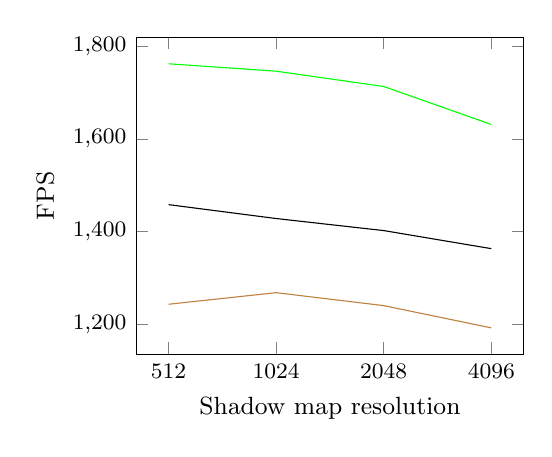
\begin{tikzpicture}
        \begin{semilogxaxis}[
            small,
            xlabel={Shadow map resolution},
            ylabel={FPS},
            xtick={512,1024,2048,4096},
            xticklabels={512,1024,2048,4096},
            % legend style={
            %     overlay,
            %     at={(1.25,0.5)},
            %     anchor=center},
            y tick label style={
                /pgf/number format/.cd,
                    fixed,   % po zakomentowaniu os rzednych jest indeksowana wykladniczo
                    fixed, % 1.0 zamiast 1
                    precision=1,
                /tikz/.cd
            },
            x tick label style={
                /pgf/number format/.cd,
                    fixed,
                    fixed,
                    precision=2,
                /tikz/.cd
            }
            ]
            \addplot [color=green]
            coordinates {
                (512,1762)(1024,1746)(2048,1713)(4096,1631)}; %\addlegendentry{720p}
            \addplot [color=black]
            coordinates {
                (512,1458)(1024,1428)(2048,1402)(4096,1363)}; %\addlegendentry{1080p}
            \addplot [color=brown]
            coordinates {
                (512,1243)(1024,1268)(2048,1240)(4096,1192)}; %\addlegendentry{2k}
        \end{semilogxaxis} 
    \end{tikzpicture}
    \caption{Results for Chinese Dragon scene.}
    \label{fig:plot:basic_dragon}
\end{subfigure}
\hfill
\begin{subfigure}[t]{0.48\textwidth}
    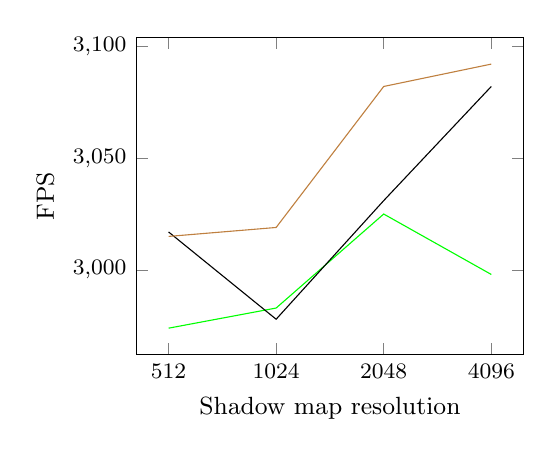
\begin{tikzpicture}
        \begin{semilogxaxis}[
            small,
            xlabel={Shadow map resolution},
            ylabel={FPS},
            xtick={512,1024,2048,4096},
            xticklabels={512,1024,2048,4096},
            % legend style={
            %     overlay,
            %     at={(1.25,0.5)},
            %     anchor=center},
            y tick label style={
                /pgf/number format/.cd,
                    fixed,   % po zakomentowaniu os rzednych jest indeksowana wykladniczo
                    fixed, % 1.0 zamiast 1
                    precision=1,
                /tikz/.cd
            },
            x tick label style={
                /pgf/number format/.cd,
                    fixed,
                    fixed,
                    precision=2,
                /tikz/.cd
            }
            ]
            \addplot [color=green]
            coordinates {
                (512,2974)(1024,2983)(2048,3025)(4096,2998)}; %\addlegendentry{720p}
            \addplot [color=black]
            coordinates {
                (512,3017)(1024,2978)(2048,3031)(4096,3082)}; %\addlegendentry{1080p}
            \addplot [color=brown]
            coordinates {
                (512,3015)(1024,3019)(2048,3082)(4096,3092)}; %\addlegendentry{2k}
        \end{semilogxaxis} 
    \end{tikzpicture}
    \caption{Results for the Cube scene.}
    \label{fig:plot:basic_cube}
\end{subfigure}

\vspace{20pt}
\begin{subfigure}[t]{0.48\textwidth}
    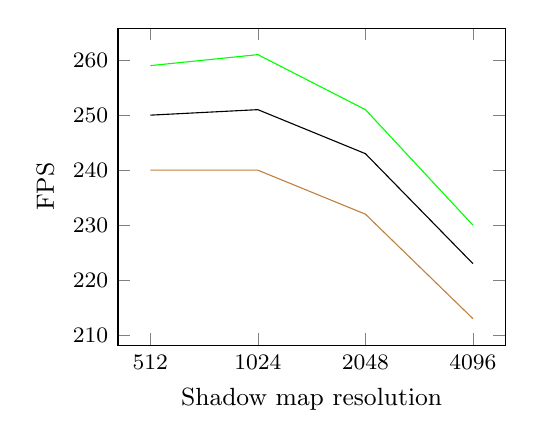
\begin{tikzpicture}
        \begin{semilogxaxis}[
            small,
            xlabel={Shadow map resolution},
            ylabel={FPS},
            xtick={512,1024,2048,4096},
            xticklabels={512,1024,2048,4096},
            % legend style={
            %     overlay,
            %     at={(1.25,0.5)},
            %     anchor=center},
            y tick label style={
                /pgf/number format/.cd,
                    fixed,   % po zakomentowaniu os rzednych jest indeksowana wykladniczo
                    fixed, % 1.0 zamiast 1
                    precision=1,
                /tikz/.cd
            },
            x tick label style={
                /pgf/number format/.cd,
                    fixed,
                    fixed,
                    precision=2,
                /tikz/.cd
            }
            ]
            \addplot [color=green]
            coordinates {
                (512,259)(1024,261)(2048,251)(4096,230)}; %\addlegendentry{720p}
            \addplot [color=black]
            coordinates {
                (512,250)(1024,251)(2048,243)(4096,223)}; %\addlegendentry{1080p}
            \addplot [color=brown]
            coordinates {
                (512,240)(1024,240)(2048,232)(4096,213)}; %\addlegendentry{2k}
        \end{semilogxaxis} 
    \end{tikzpicture}
    \caption{Results for the Power Plant scene.}
    \label{fig:plot:basic_power}
\end{subfigure}
\hfill
\begin{subfigure}[t]{0.48\textwidth}
    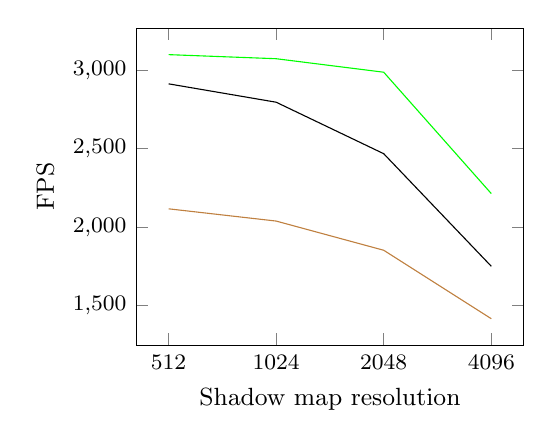
\begin{tikzpicture}
        \begin{semilogxaxis}[
            small,
            xlabel={Shadow map resolution},
            ylabel={FPS},
            xtick={512,1024,2048,4096},
            xticklabels={512,1024,2048,4096},
            % legend style={
            %     overlay,
            %     at={(1.25,0.5)},
            %     anchor=center},
            y tick label style={
                /pgf/number format/.cd,
                    fixed,   % po zakomentowaniu os rzednych jest indeksowana wykladniczo
                    fixed, % 1.0 zamiast 1
                    precision=1,
                /tikz/.cd
            },
            x tick label style={
                /pgf/number format/.cd,
                    fixed,
                    fixed,
                    precision=2,
                /tikz/.cd
            }
            ]
            \addplot [color=green]
            coordinates {
                (512,3098)(1024,3072)(2048,2986)(4096,2213)}; %\addlegendentry{720p}
            \addplot [color=black]
            coordinates {
                (512,2912)(1024,2795)(2048,2467)(4096,1750)}; %\addlegendentry{1080p}
            \addplot [color=brown]
            coordinates {
                (512,2116)(1024,2038)(2048,1852)(4096,1416)}; %\addlegendentry{2k}
        \end{semilogxaxis} 
    \end{tikzpicture}
    \caption{Results for the Crytek Sponza scene.}
    \label{fig:plot:basic_sponza}
\end{subfigure}
\caption{Frames per second for all test scenes, for different sizes of the shadow map and output resolutions. In green \(1280\times 720\), in black \(1920\times 1080\) and in brown \(2560\times 1440\).}
\label{fig:plot:basic_results}
\end{figure}

The test results mostly match the expectation that fewer FPS will be produced with increasing shadow map resolution and output resolution. The only exception is plot \ref{fig:plot:basic_cube} of the Cube scene results. This is however probably due to the fact that this scene is so simple, and in effect is rendered with such high FPS (highest in this test set, over 3000), that any interruptions from other programs on the machine will be visible. Inconsistencies might also be produced by hardware cores' dynamic clock rates, which can vary over the duration of the test.

The basic shadow mapping algorithm is simple enough to produce high FPS. Even in the most complex scene, the Power Plant, over 210 frames are rendered at 2k output and 4k shadow map resolution.

Looking at the shapes of the plots, it can be said that the basic shadow mapping algorithm is not dependent on output resolution. The lower FPS for higher output resolutions stem mostly from the sole fact that more pixel need to be rendered, because the FPS falloffs along the x-axis follow the same shape. In most cases the drop in FPS between the lowest and highest shadow map resolution is the same, regardless of the output resolution. 

The plots have their x-axis in logarithmic scale. Taking that into account, it can be observed that the FPS counts fall linearly with growing shadow map resolutions.

The algorithm's performance is not view-dependent. When traversing the scene the frame rates are stable. This is backed by the fact that in basic shadow mapping the same work is performed for each rendered pixel, consisting of a comparison operation with the depth value stored in the depth map. This however would not be true if shadow map fitting was used. In such case, the performance will become view dependent as more or less geometry will be rendered into the shadow map. This can provide a useful performance boost in large scenes.

Using the Tracy profiler it can be confirmed that the renderer's performance is limited by the computations performed on the GPU, as the CPU thread spent approximately \(30\%\) of time waiting for the GPU resources to be available. Tracy also reports that approximately \(40\%\) of the frame time was spent on the shadow map render pass and \(52\%\) on the main render pass. The remaining time was spent rendering the GUI and synchronizing. This can be expected as with this simple technique the shadow map pass is almost as expensive as the main pass. The main pass is slightly more involved as it outputs pixels and performs simple shading, as well as performs the shadow mapping itself, which requires texture lookups and comparisons that add time.

The rendering results for the Chinese Dragon are presented in Fig. \ref{fig:test_basic_dragon_screens} and in Fig. \ref{fig:test_basic_sponza_screens} the Crytek Sponza is presented.
\begin{figure}
    \centering
    \begin{subfigure}{0.48\textwidth}
		\centering
        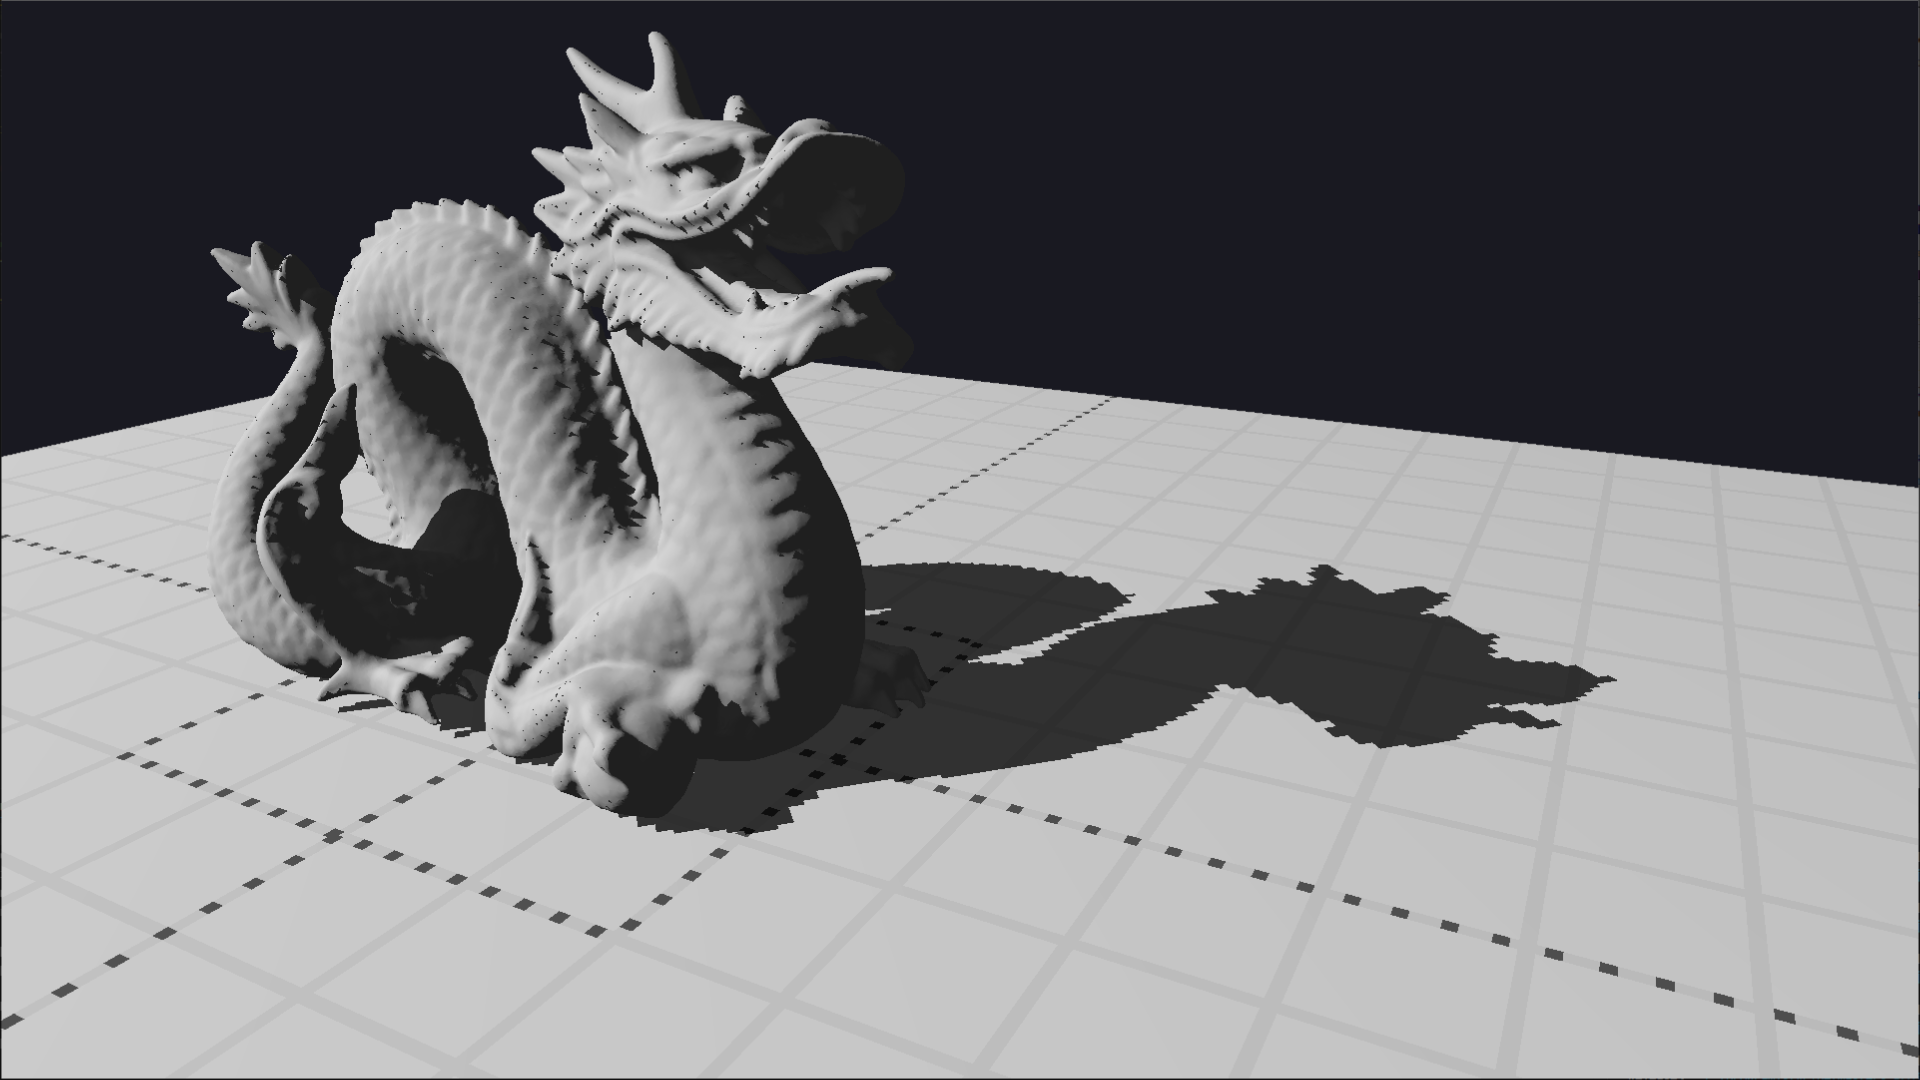
\includegraphics[width=\textwidth]{./graf/tests/basic/cropped/dragon_basic_fhd_512.png}
        \caption{The Chinese Dragon rendered with \(512\times 512\) shadow map.}
    \end{subfigure}
	\hfill
    \begin{subfigure}{0.48\textwidth}
		\centering
        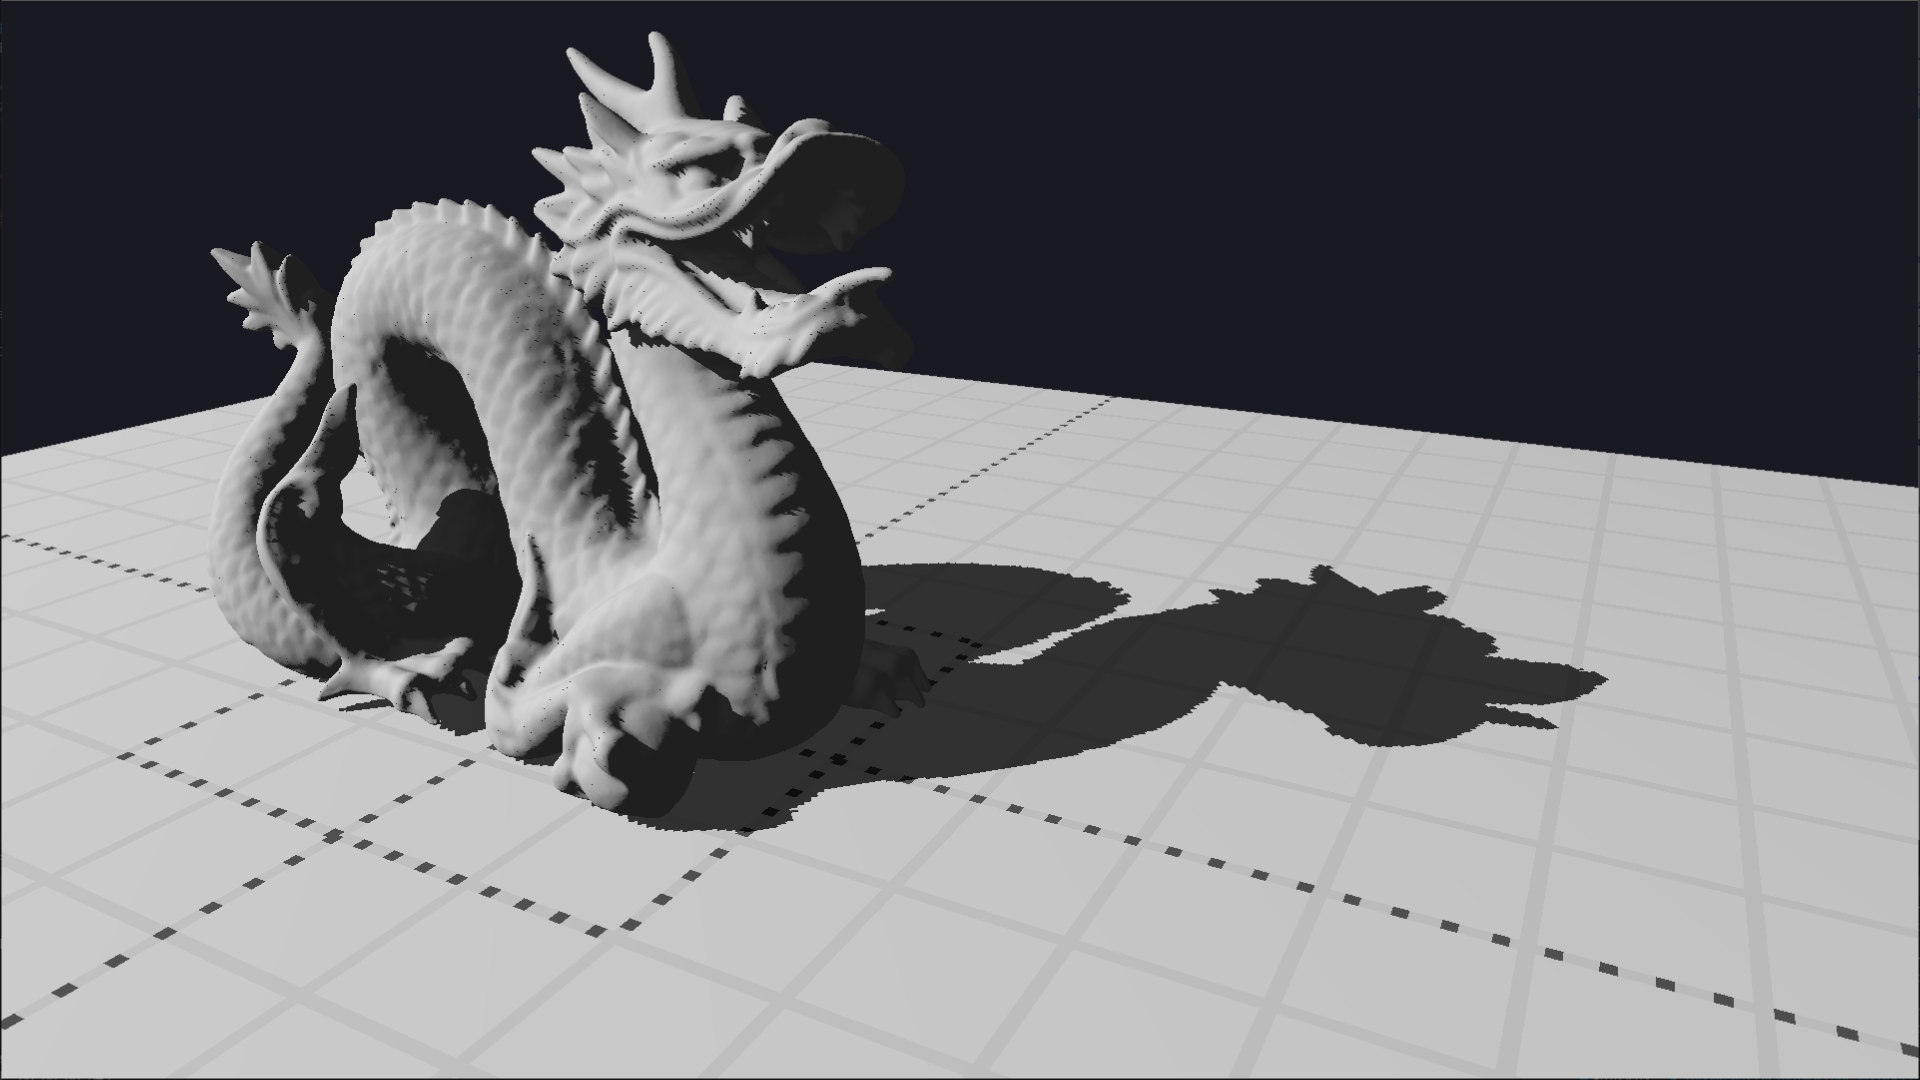
\includegraphics[width=\textwidth]{./graf/tests/basic/cropped/dragon_basic_fhd_1024.png}
        \caption{The Chinese Dragon rendered with \(1024\times 1024\) shadow map.}
    \end{subfigure}

    \begin{subfigure}{0.48\textwidth}
		\centering
        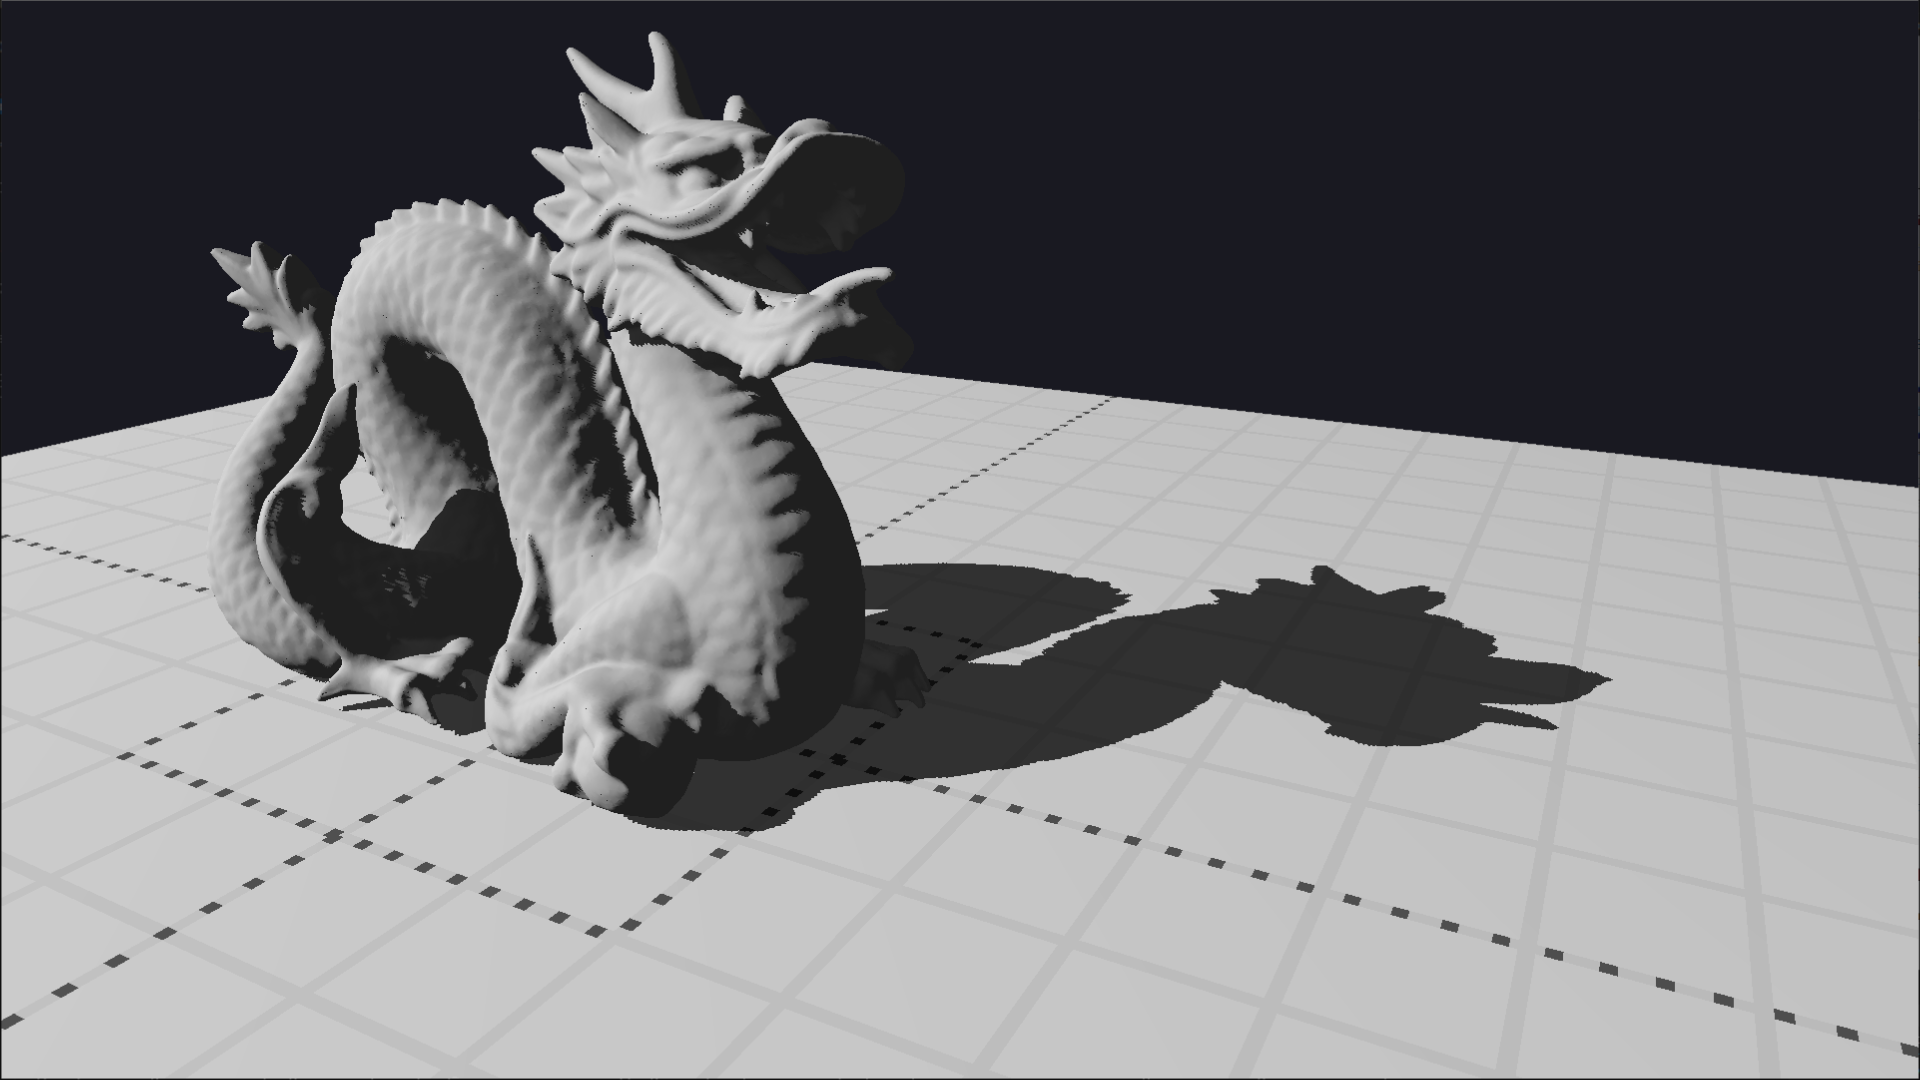
\includegraphics[width=\textwidth]{./graf/tests/basic/cropped/dragon_basic_fhd_2048.png}
        \caption{The Chinese Dragon rendered with \(2048\times 2048\) shadow map.}
    \end{subfigure}
	\hfill
    \begin{subfigure}{0.48\textwidth}
		\centering
        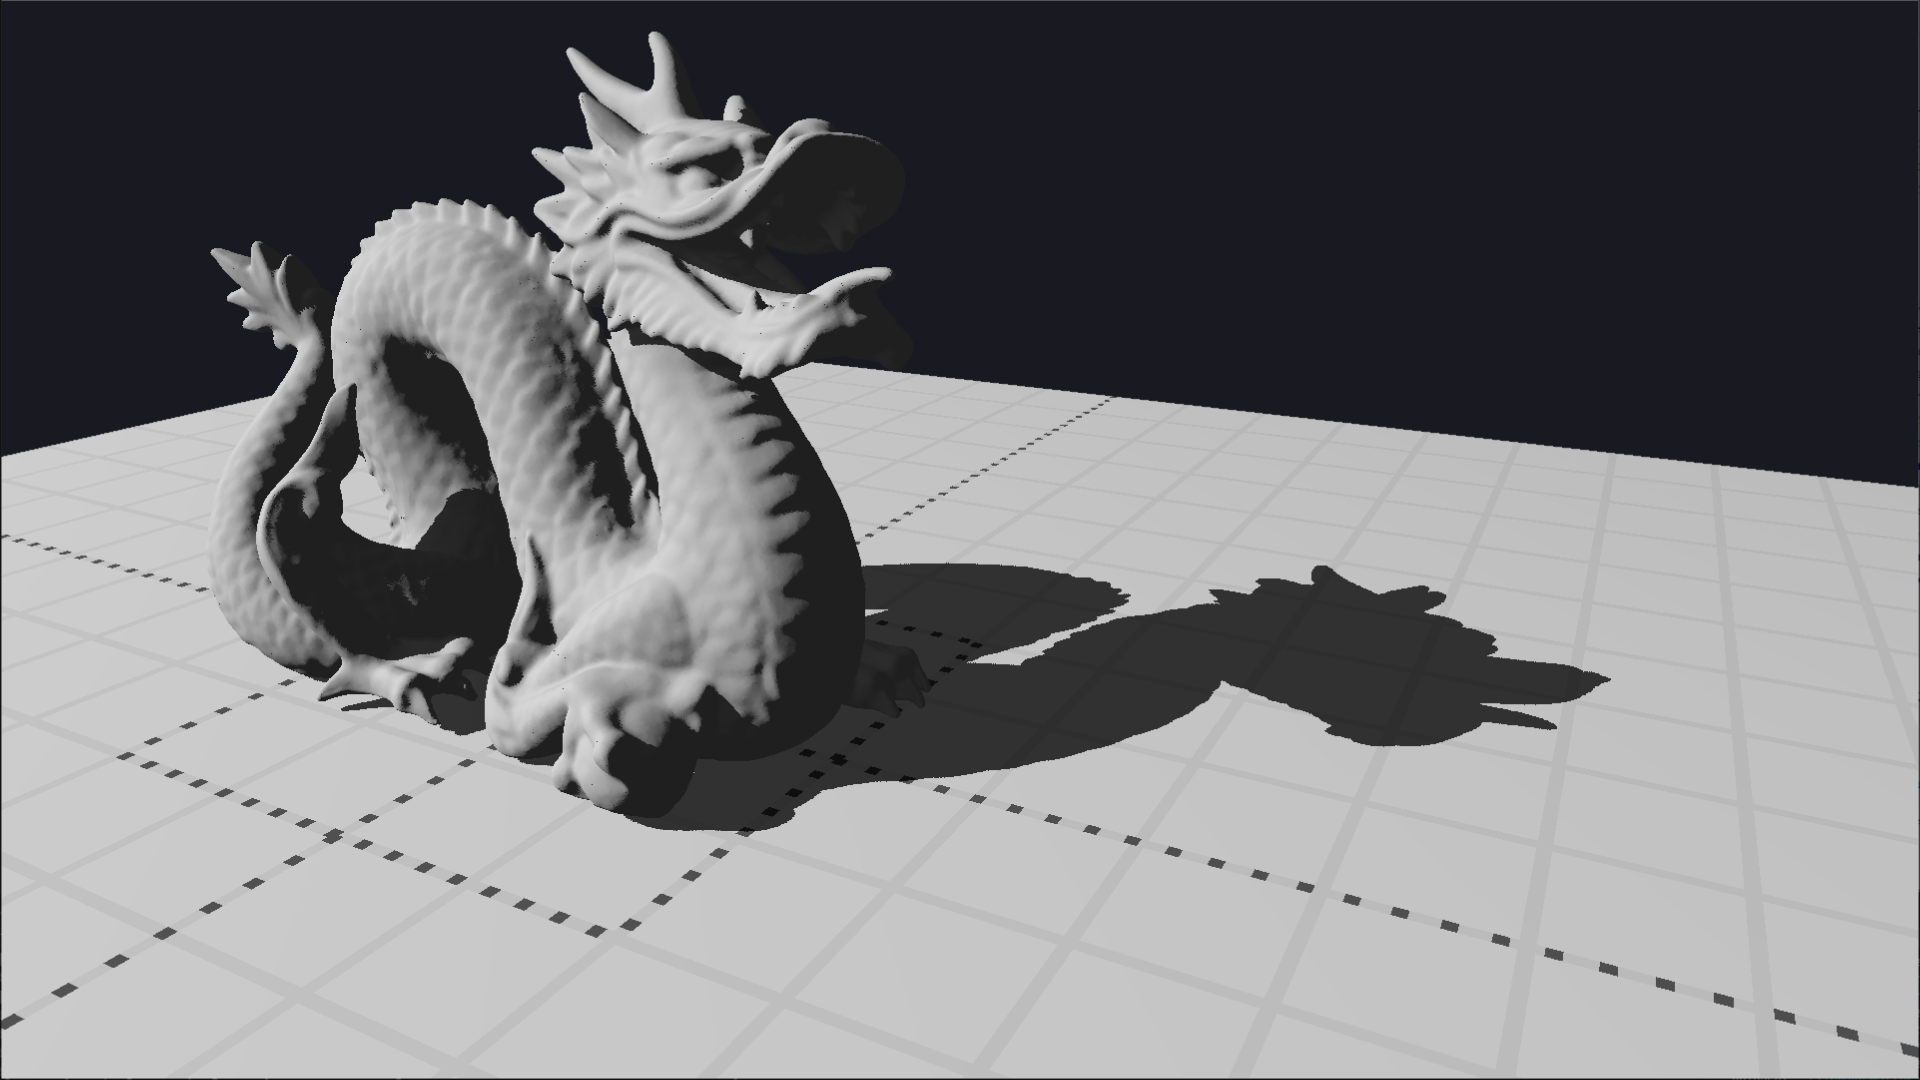
\includegraphics[width=\textwidth]{./graf/tests/basic/cropped/dragon_basic_fhd_4096.png}
        \caption{The Chinese Dragon rendered with \(4096\times 4096\) shadow map.}
    \end{subfigure}

    \caption{The Chinese Dragon scene rendered with different shadow map resolutions, using the basic shadow mapping algorithm.}
    \label{fig:test_basic_dragon_screens}
\end{figure}
\begin{figure}
    \centering
    \begin{subfigure}{0.48\textwidth}
		\centering
        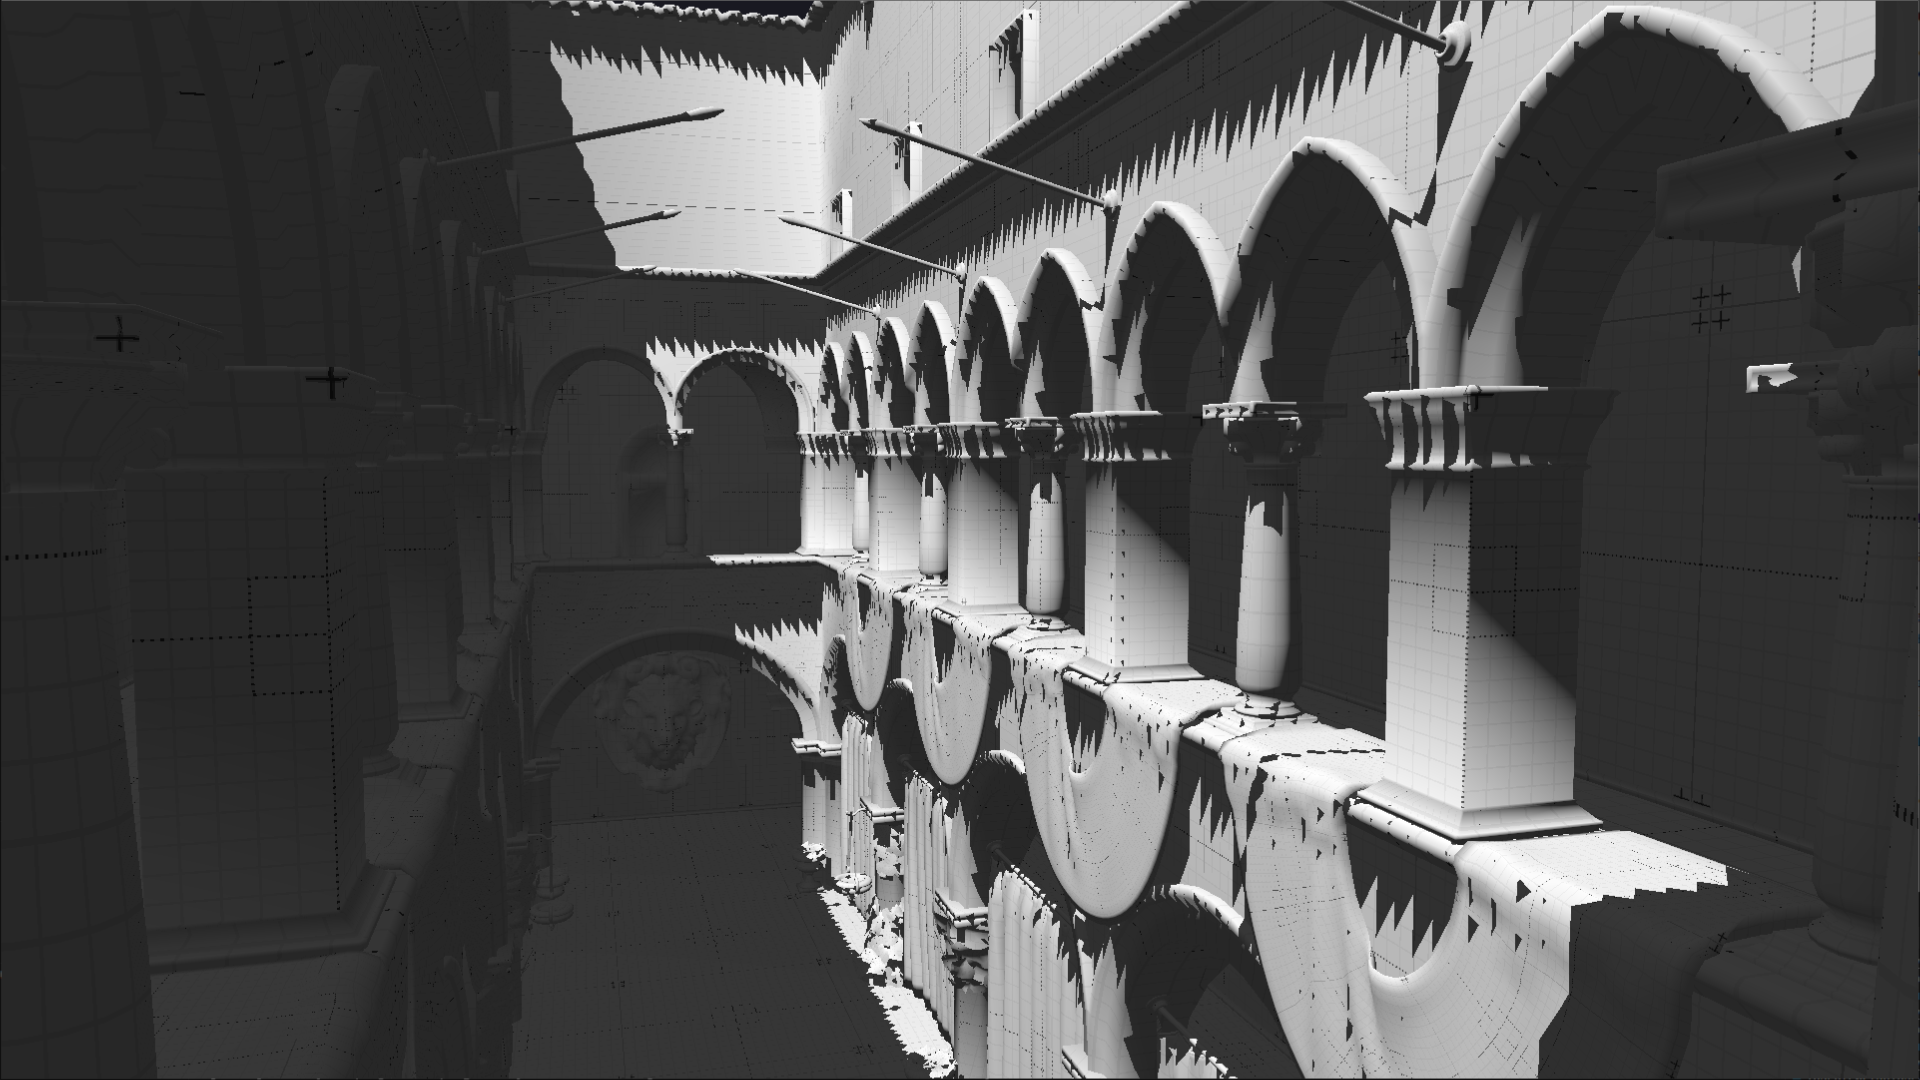
\includegraphics[width=\textwidth]{./graf/tests/basic/cropped/sponza_basic_fhd_512.png}
        \caption{The Crytek Sponza rendered with \(512\times 512\) shadow map.}
    \end{subfigure}
	\hfill
    \begin{subfigure}{0.48\textwidth}
		\centering
        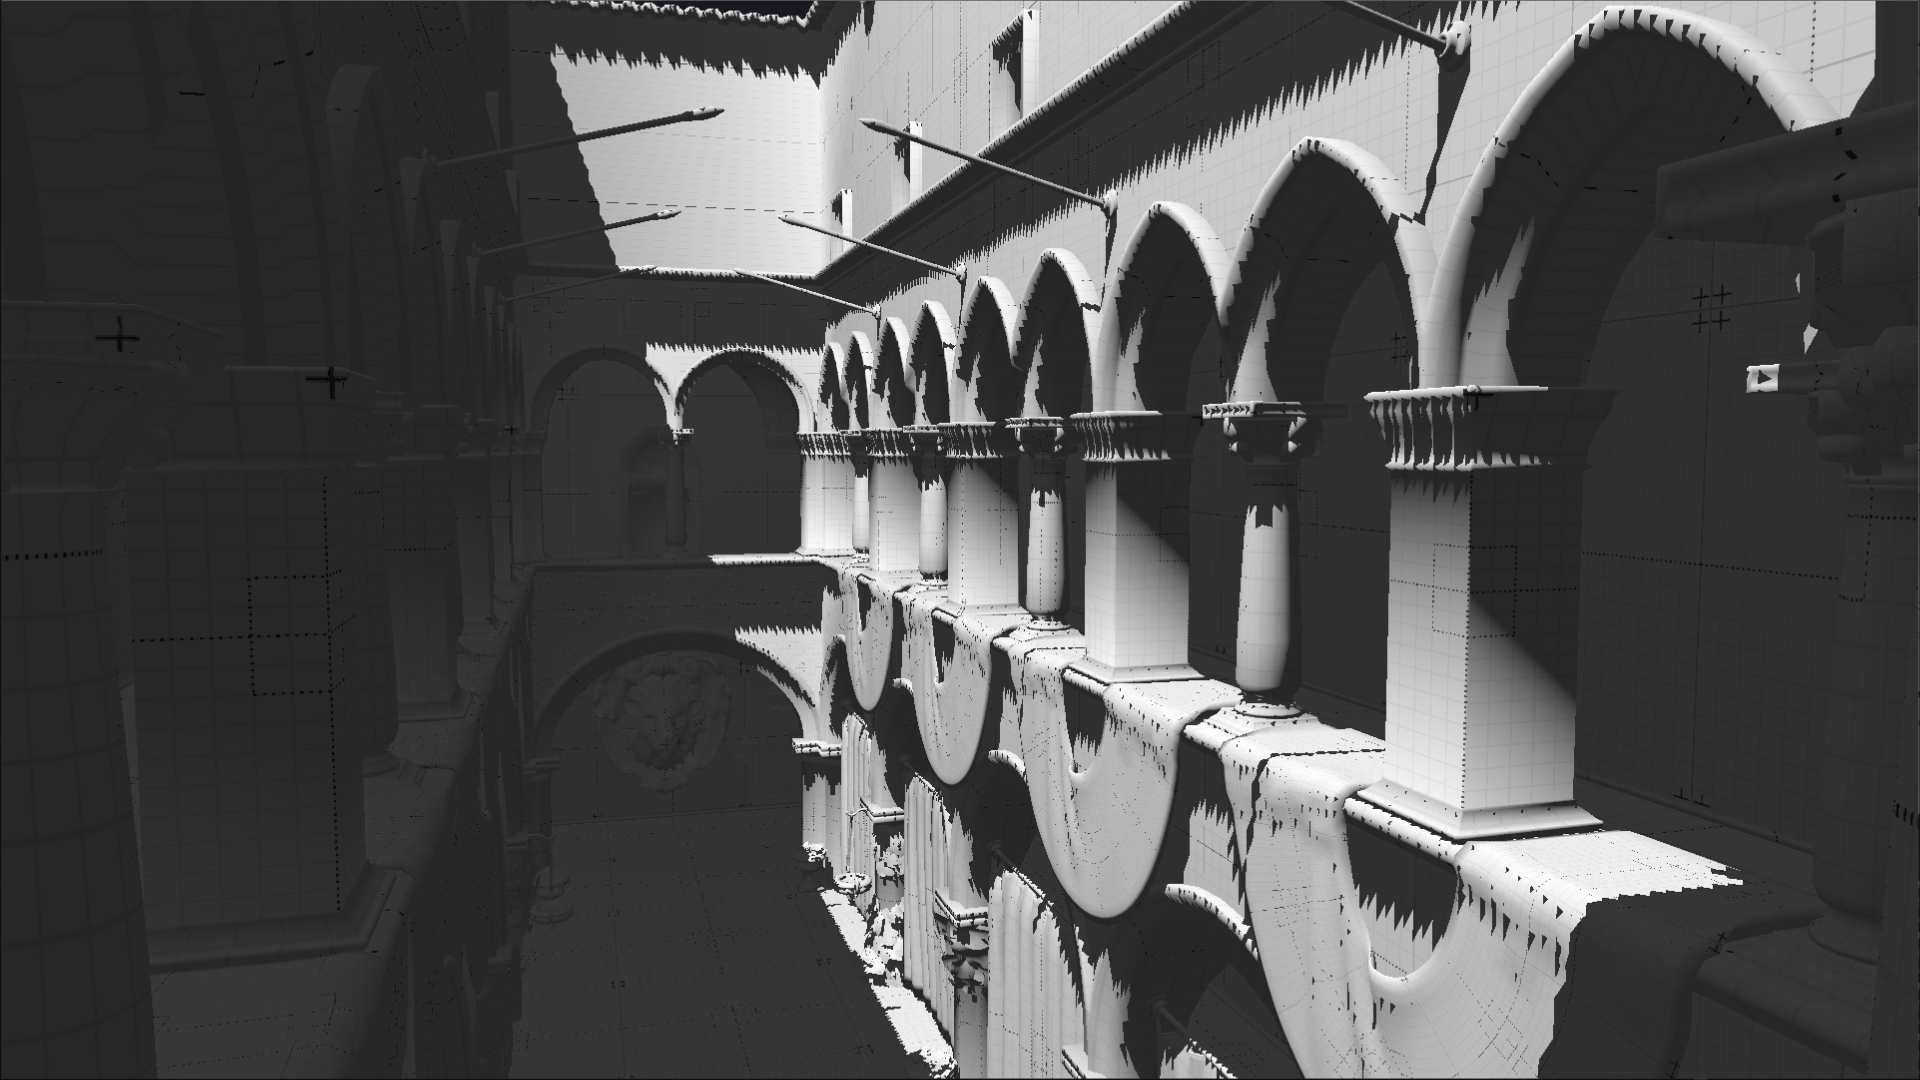
\includegraphics[width=\textwidth]{./graf/tests/basic/cropped/sponza_basic_fhd_1024.png}
        \caption{The Crytek Sponza rendered with \(1024\times 1024\) shadow map.}
    \end{subfigure}

    \begin{subfigure}{0.48\textwidth}
		\centering
        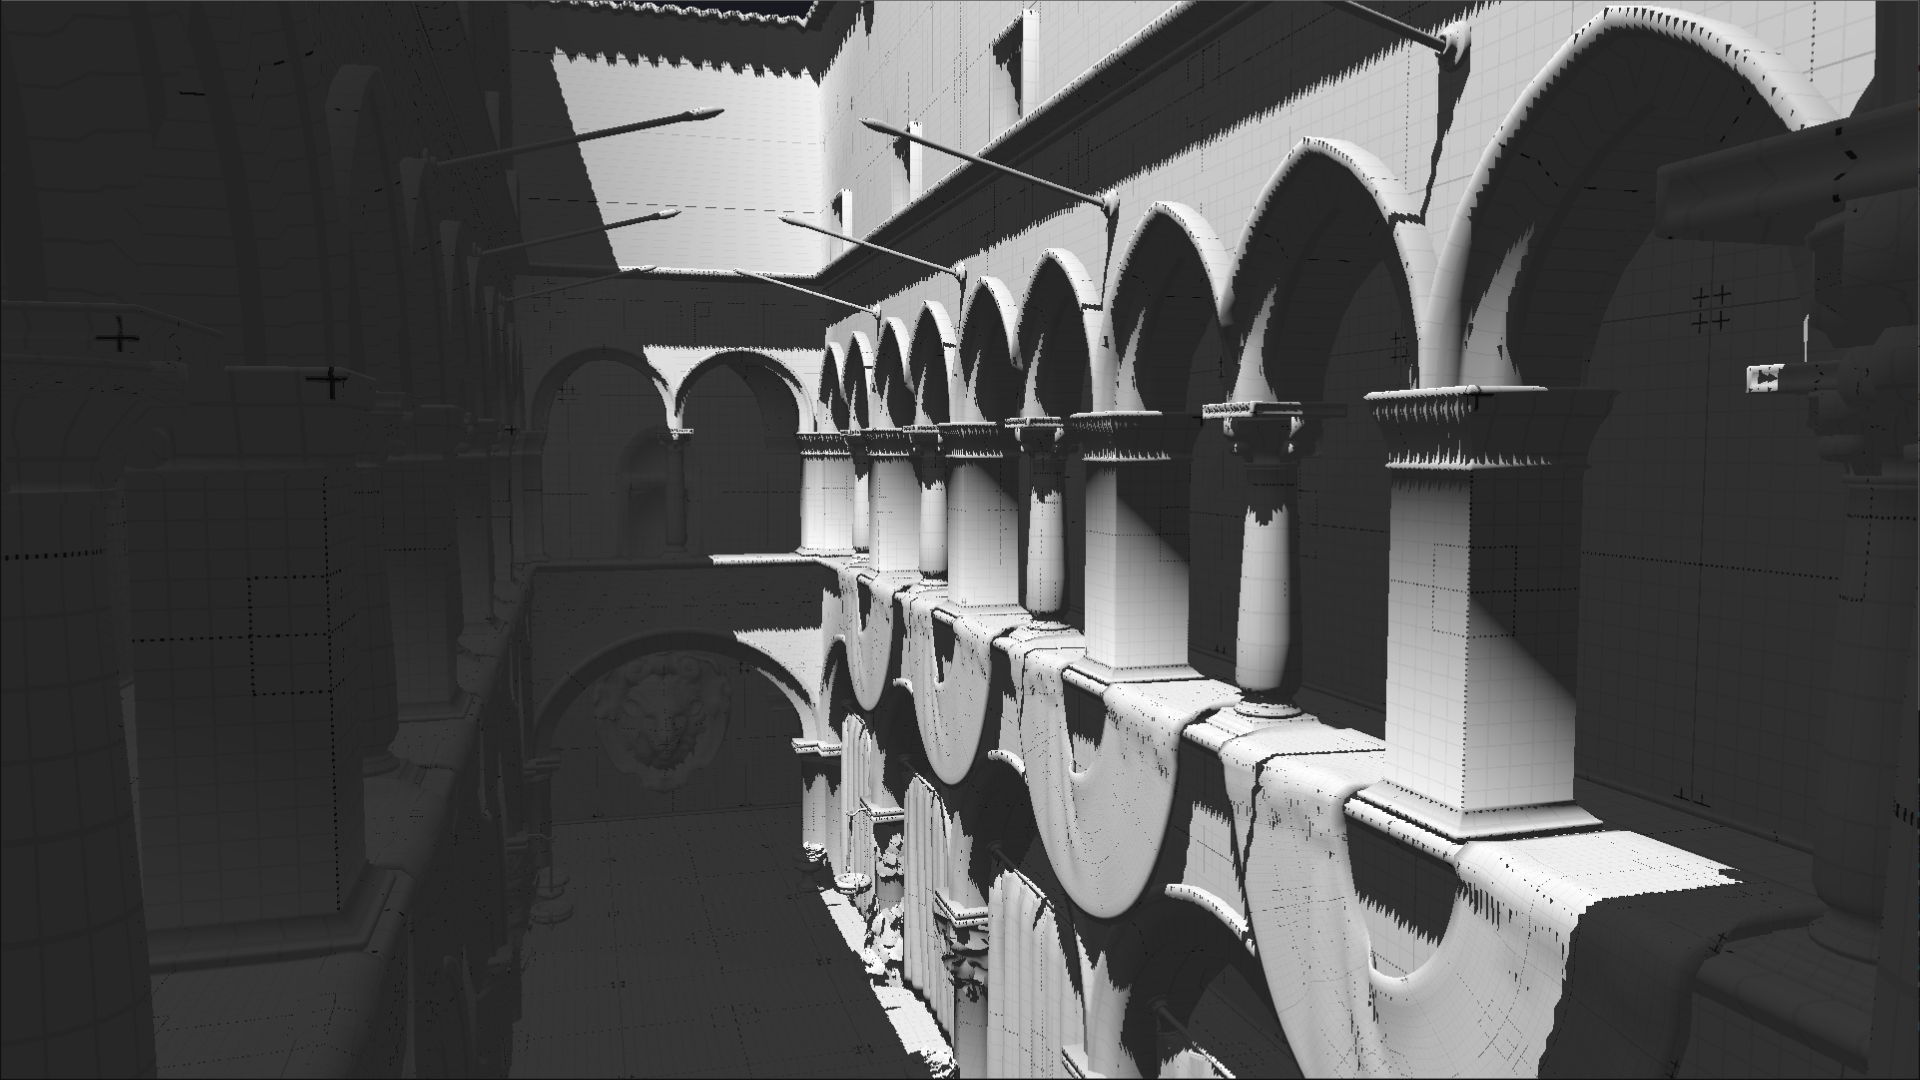
\includegraphics[width=\textwidth]{./graf/tests/basic/cropped/sponza_basic_fhd_2048.png}
        \caption{The Crytek Sponza rendered with \(2048\times 2048\) shadow map.}
    \end{subfigure}
	\hfill
    \begin{subfigure}{0.48\textwidth}
		\centering
        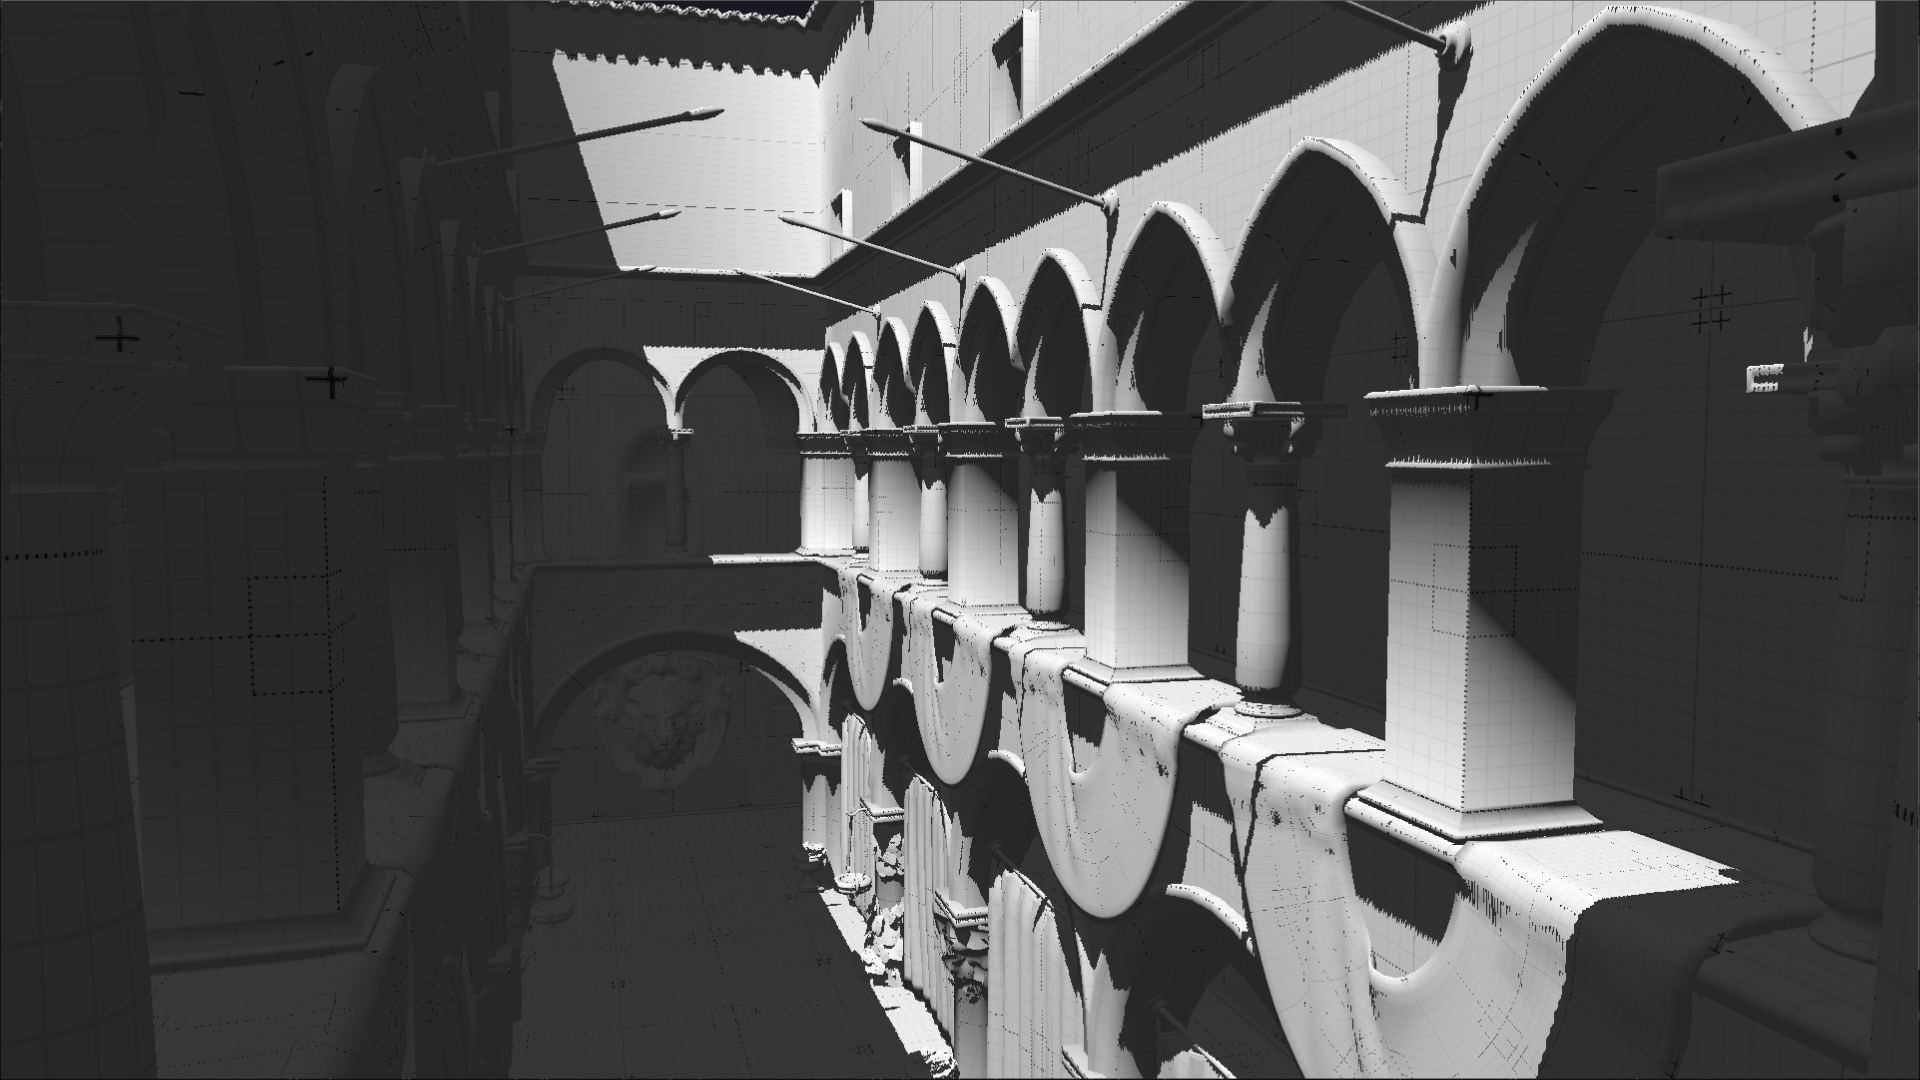
\includegraphics[width=\textwidth]{./graf/tests/basic/cropped/sponza_basic_fhd_4096.png}
        \caption{The Crytek Sponza rendered with \(4096\times 4096\) shadow map.}
    \end{subfigure}

    \caption{The Crytek Sponza scene rendered with different shadow map resolutions, using the basic shadow mapping algorithm.}
    \label{fig:test_basic_sponza_screens}
\end{figure}

The Chinese Dragon results are quite good for higher resolution shadow maps, since the shadow map texels map many to one with regard to screen pixels. Aliasing is however very visible for lower resolutions. Crytek Sponza suffers from shadow acne on vertical surfaces. This is a sign of badly chosen shadow bias. It gets less visible as resolution rises, but is always present. Even at the highest resolution, shadow map texel borders are still visible, where they were not visible in the Chinese Dragon scene. This is due to the fact that the shadow map covers a larger area and each shadow map texel covers more space on the screen.

\subsection{Filtered shadow maps}

\subsubsection{Hardware bilinear filtering}

\subsubsection{Percentage-closer filtering}

\subsubsection{PCF with bilinear filtering}

\subsubsection{Adaptive percentage-closer filtering}

\subsection{Soft shadows with shadow maps}

\subsubsection{PCSS}

% \begin{table}
% \centering
% \caption{A caption of a table is ABOVE it.}
% \label{id:tab:wyniki}
% \begin{tabular}{rrrrrrrr}
% \toprule
% 	         &                                     \multicolumn{7}{c}{method}                                      \\
% 	         \cmidrule{2-8}
% 	         &         &         &        \multicolumn{3}{c}{alg. 3}        & \multicolumn{2}{c}{alg. 4, $\gamma = 2$} \\
% 	         \cmidrule(r){4-6}\cmidrule(r){7-8}
% 	$\zeta$ &     alg. 1 &   alg. 2 & $\alpha= 1.5$ & $\alpha= 2$ & $\alpha= 3$ &   $\beta = 0.1$  &   $\beta = -0.1$ \\
% \midrule
% 	       0 &  8.3250 & 1.45305 &       7.5791 &    14.8517 &    20.0028 & 1.16396 &                       1.1365 \\
% 	       5 &  0.6111 & 2.27126 &       6.9952 &    13.8560 &    18.6064 & 1.18659 &                       1.1630 \\
% 	      10 & 11.6126 & 2.69218 &       6.2520 &    12.5202 &    16.8278 & 1.23180 &                       1.2045 \\
% 	      15 &  0.5665 & 2.95046 &       5.7753 &    11.4588 &    15.4837 & 1.25131 &                       1.2614 \\
% 	      20 & 15.8728 & 3.07225 &       5.3071 &    10.3935 &    13.8738 & 1.25307 &                       1.2217 \\
% 	      25 &  0.9791 & 3.19034 &       5.4575 &     9.9533 &    13.0721 & 1.27104 &                       1.2640 \\
% 	      30 &  2.0228 & 3.27474 &       5.7461 &     9.7164 &    12.2637 & 1.33404 &                       1.3209 \\
% 	      35 & 13.4210 & 3.36086 &       6.6735 &    10.0442 &    12.0270 & 1.35385 &                       1.3059 \\
% 	      40 & 13.2226 & 3.36420 &       7.7248 &    10.4495 &    12.0379 & 1.34919 &                       1.2768 \\
% 	      45 & 12.8445 & 3.47436 &       8.5539 &    10.8552 &    12.2773 & 1.42303 &                       1.4362 \\
% 	      50 & 12.9245 & 3.58228 &       9.2702 &    11.2183 &    12.3990 & 1.40922 &                       1.3724 \\
% \bottomrule
% \end{tabular}
% \end{table}  

% The table is here too \ref{id:tab:wyniki}

%%%%%%%%%%%%%%%%%%%%%
% FIGURE FROM FILE
%
% \begin{figure}
% \centering
% 
\includegraphics[width=0.5\textwidth]{./graf/politechnika_sl_logo_bw_pion_en.pdf}
% \caption{Caption of a figure is always below the figure.}
% \label{fig:label}
% \end{figure}

% Fig. \ref{fig:label} presents asdasd

% \begin{figure}
% 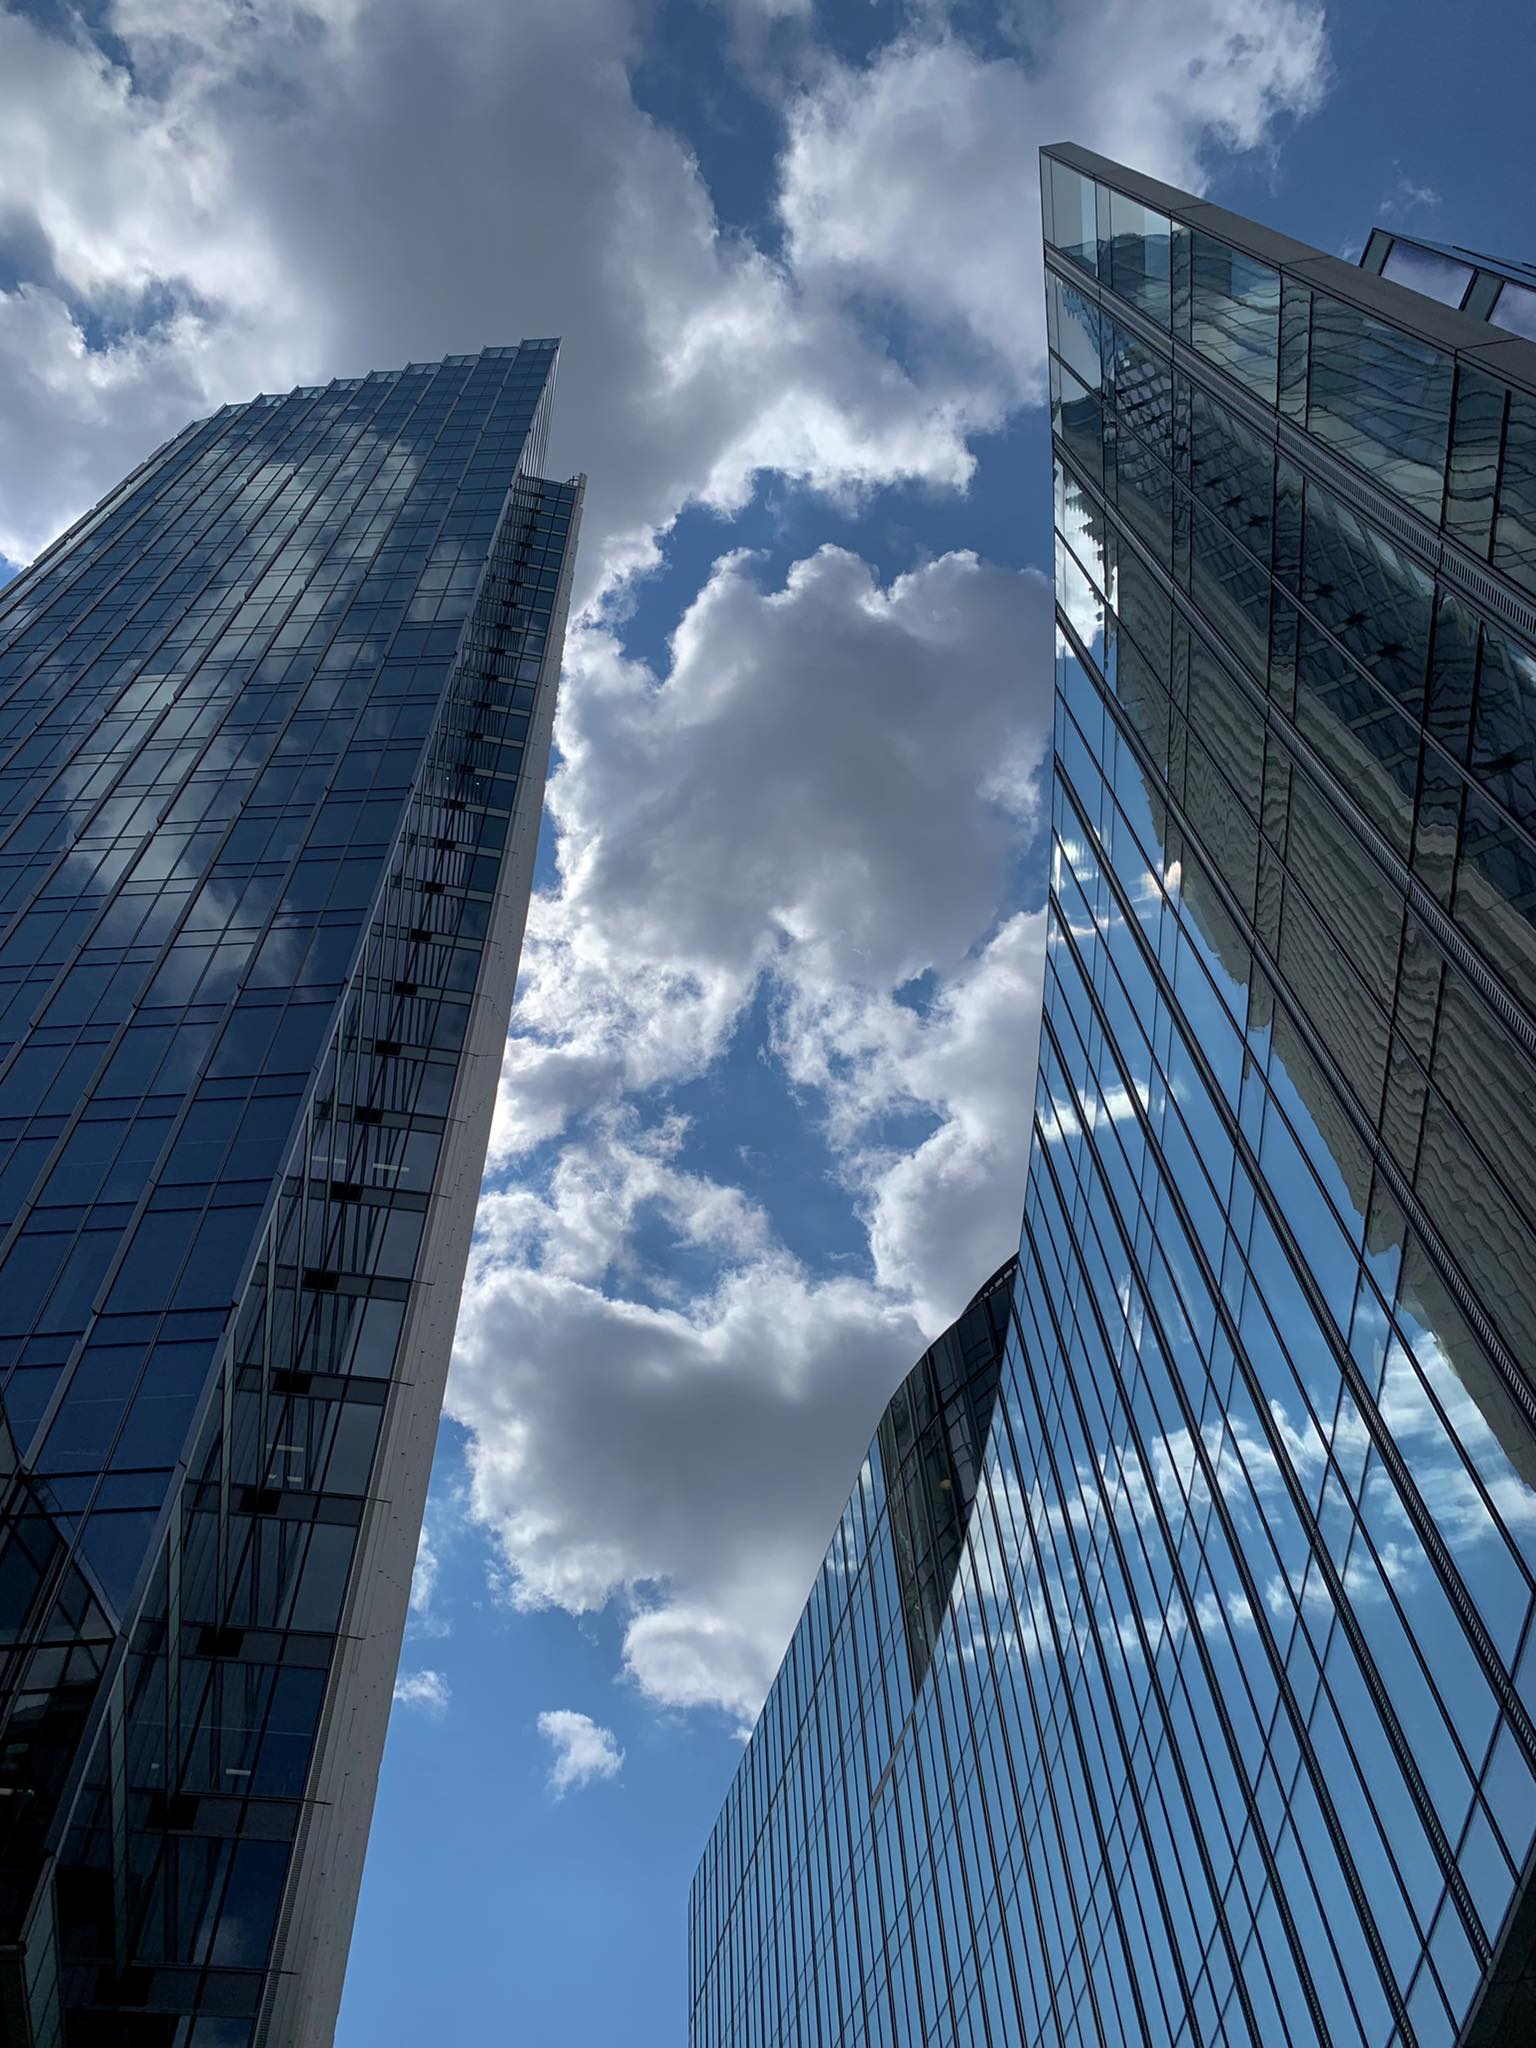
\includegraphics[width=0.5\textwidth]{./graf/test_image.jpg}
% \caption{Caption of a figure is always below the figure akakak.}
% \label{fig:duped_image3}
% \end{figure}

% some citation of the above \ref{fig:duped_image3}

%%%%%%%%%%%%%%%%%%%%%
%
%%%%%%%%%%%%%%%%%%%%
%% SUBFIGURES
%
% \begin{figure}
% \centering
% \begin{subfigure}{0.4\textwidth}
%    
\includegraphics[width=\textwidth]{./graf/politechnika_sl_logo_bw_pion_en.pdf}
%    \caption{Upper left figure.}
%    \label{fig:upper-left}
% \end{subfigure}
% \hfill
% \begin{subfigure}{0.4\textwidth}
%    
\includegraphics[width=\textwidth]{./graf/politechnika_sl_logo_bw_pion_en.pdf}
%    \caption{Upper right figure.}
%    \label{fig:upper-right}
% \end{subfigure}

% \begin{subfigure}{0.4\textwidth}
%    
\includegraphics[width=\textwidth]{./graf/politechnika_sl_logo_bw_pion_en.pdf}
%    \caption{Lower left figure.}
%    \label{fig:lower-left}
% \end{subfigure}
% \hfill
% \begin{subfigure}{0.4\textwidth}
%    
\includegraphics[width=\textwidth]{./graf/politechnika_sl_logo_bw_pion_en.pdf}
%    \caption{Lower right figure.}
%    \label{fig:lower-right}
% \end{subfigure}
       
% \caption{Common caption for all subfigures.}
% \label{fig:subfigures}
% \end{figure}
% Fig. \ref{fig:subfigures} presents very important information, eg. Fig. \ref{fig:upper-right} is an upper right subfigure.
%%%%%%%%%%%%%%%%%%%%%



% \begin{figure}
% \centering
% \begin{tikzpicture}
% \begin{axis}[
%    y tick label style={
%        /pgf/number format/.cd,
%            fixed,   % po zakomentowaniu os rzednych jest indeksowana wykladniczo
%            fixed zerofill, % 1.0 zamiast 1
%            precision=1,
%        /tikz/.cd
%    },
%    x tick label style={
%        /pgf/number format/.cd,
%            fixed,
%            fixed zerofill,
%            precision=2,
%        /tikz/.cd
%    }
% ]
% \addplot [domain=0.0:0.1] {rnd};
% \end{axis} 
% \end{tikzpicture}
% \caption{Figure caption is BELOW the figure.}
% \label{fig:3}
% \end{figure}

% \begin{figure}
% \centering
% 
\includegraphics[width=0.5\textwidth]{./graf/politechnika_sl_logo_bw_pion_en.pdf}
% \caption{Caption of a figure is always below the figure akakak.}
% \label{fig:3}
% \end{figure}

% some citation of the above \ref{fig:3}

% \begin{figure}
% \begin{lstlisting}
% if (_nClusters < 1)
% 	throw std::string ("unknown number of clusters");
% if (_nIterations < 1 and _epsilon < 0)
% 	throw std::string ("You should set a maximal number of iteration or minimal difference -- epsilon.");
% if (_nIterations > 0 and _epsilon > 0)
% 	throw std::string ("Both number of iterations and minimal epsilon set -- you should set either number of iterations or minimal epsilon.");
% \end{lstlisting}
% \caption{Example of pseudocode.}
% \end{figure}